\chapter{Dynkin Diagrams}
\label{ch-dynkin}

\newcommand{\valp}[0]{{\vec{\alp}}}
\newcommand{\vbeta}[0]{{\vec{\beta}}}
\newcommand{\vgamma}[0]{{\vec{\gamma}}}

This chapter is based on Ref.\cite{eli-daw-book}, section 20.4.

This chapter is an overview of the classification
of simple Lie Algebras invented mainly by Killing, Cartan and Dynkin, in that historical order. This classification is valid for Lie Algebras over $\CC$\footnote{More generally, Cartan's classification is valid for Lie Algebras over $\FF$, where $\FF$ is an algebraically closed field of characteristic zero.} This distinction is important because there are many more simple Lie algebras over $\RR$ than over $\CC$. When defining the generators of Lie Algebras in other chapters, we defined a real Lie Algebra $\ger{g}_\RR$ (a vector space over $\RR$)
which exponentiates to a group $\calg_\RR=\exp(\ger{g}_\RR)$.
This chapter refers to the complexification
$\ger{g}_\CC$ of $\ger{g}_\RR$ (complex vector space)
and to the group $\calg_\CC=\exp(\ger{g}_\CC)$


Lie algebra $\ger{g}_\CC$ over complex numbers (complex vector space over generators $X_r$ for
$r=1,2, \ldots \cald$) $\cald=\frac{1}{2}\dim_\RR \ger{g}_\CC=\dim_\CC \ger{g}_\CC=$  half the number  of real degrees of freedom
of the Lie Algebra
\beq
[X_q, X_p] = \sum_t f\indices{_q_p^t}X_t
\eeq



\beq
g_{qs}= \sum_{p,t}f\indices{_q_p^t}
f\indices{_s_t^p}
=
\bcen
\xymatrix{
q\ar@{~}[r]
&f\ar@/_1pc/@{~}[r]
\ar@/^1pc/@{~}[r]
&f\ar@{~}[r]
&s
}
\ecen
\eeq

If $\det g =0$,

\beq
[X_{a}, X_{b}] = 0,
\quad
[X_q, X_p] =\sum_t f\indices{_q_p^t}X_t
\eeq

Can assume $\det g \neq 0$,
Cartan criterion (CC) for
group to be semi-simple.
If the CC is satisfied, can assume
$g_{st}$ is diagonal

\beq g_{s t}=\delta(s,t)=
\xymatrix{
\ar@{~}[r]&
}
\eeq

\beq
f\indices{_q_p^t}=f_{qpt}
\eeq
Will not choose $f_{qpt}$
to be totally antisymmetric


$q_- = 1, 2, \ldots,\calr$

$\valp = 1,2, \ldots, 
\cald-\calr$ 

$q=$ either $q_-$ or $\valp$ but not both.



Let $\{H_{i_-}\}_{i_-=1}^\calr$
be the largest possible set
of mutually commuting $X_p$.
$\calr$ is called the {\bf rank} of the group.

\beq
\boxed{[H_{i_-}, H_{j_-}]=0}
\eeq

Choose $E_{\vec{\alp}}$
to be eigenvectors of $H_{i_-}$ in the commutator \qt{product}
\beq
\boxed{[H_{i_-}, E_{\vec{\alp}}]= \underbrace{\alp_{i_-}}_{f_{i_-,\valp,\valp}} E_{\valp}}
\eeq


Then\footnote{The commutator $[x,y]=xy-yx$ acts like a derivative operator: 
$ [x[a,b]]= [[x,a],b] + 
[a,[x,b]]$}

Root vectors $\alp\in \RR^\calr$
\beqa
[H_i, [E_\valp,
E_\vbeta]]
&=&
[[H_i, E_\valp], E_\vbeta]
+
[E_\valp, [H_i, E_\vbeta]]
\\
&=&
(\alp_i + \beta_i)[E_\valp, E_\vbeta]
\eeqa

If $\valp + \vbeta=0$,
$[H_i, [E_\valp,
E_\vbeta]]=0$ so

\beq
\boxed{[E_\valp,
E_{-\valp}] = \sum_{i_-} \underbrace{\alp^{i_-}}_{f_{\valp,-\valp,i_-}} H_{i_-}}
\eeq

If $\valp + \vbeta\neq 0$,

\beq
\boxed{[E_\valp, E_\vbeta]=
 N_{\valp,\vbeta}
E_{\valp + \vbeta}
\quad \text{ if } \valp+\vbeta \neq 0}
\eeq


\beq
\alp^{i_-}=f_{\valp,-\valp,i_-} 
\eeq

Dynking Diagram (DD)

The roots of a semisimple lie algebra form a
real vector space.

A {\bf positive/negative (P/N) root} $\valp$ is 
root for which the first component $\alp_1$ is positive/negative.
If the first component of $\valp$ is zero, then
decide the root's sign from its second component $\alp_2$. And so on.
Note that the definition of positive root is basis
dependent.

A P root $\valp$ is a {\bf simple positive (SP)
root} if there are no P roots
$\vec{\rho}$ and $\vec{\s}$ such that
$\valp= \vec{\rho}+\vec{\s}$.




Properties of root vectors $\valp, \vbeta, \ldots \in \RR^\calr$ 



\begin{enumerate}
\item If $\valp$ is a root,  then
$-\valp$ must be too.


\item We can find a basis of simple
positive roots for the root space.


\item 
\begin{claim}If $\valp$ and $\vec{\rho}$ are SP roots,
then $\valp-\vec{\rho}$ is not a root of any kind.
\end{claim}
\proof
This follows because: if $\valp-\vec{\rho}$ is a P root
 $\vec{\s} $, then
$\valp= \vec{\rho}+\vec{\s}$ so
$\valp$ is not a PS root. Likewise, if $\valp-\vec{\rho}$ is an N root $\vec{\s}$, then $-\vec{\s}$
is a P root and $\valp= \vec{\rho}+(-\vec{\s})$.
\qed



\item If $\valp$ and $\vbeta$ are PS, then there can be roots 

\beq\{\vbeta + n\valp| 
i=0, 1, 2, \ldots, n\}
\eeq
for some terminal integer $n>0$ defined by
\beq 
n= \frac{-2 \valp\cdot \vbeta}{\valp\cdot\valp}
\label{eq-dynkin-n-pic}
\eeq
Also possible are roots $\{\valp + p\vbeta| 
i=0, 1, 2, \ldots, p\}$
for some terminal integer $p>0$ defined by


\beq 
p= \frac{-2 \valp\cdot \vbeta}{\vbeta\cdot\vbeta}
\label{eq-dynkin-p-pic}
\eeq



\item angle constraints

\beq
-\sqrt{
\frac{np}{4}}
=
\hat{\alp}\cdot\hat{\beta}\in [-1, 0]
\label{eq-dynkin-angles}
\eeq


\end{enumerate}

\begin{figure}[h!]
\centering
\includegraphics[width=5in]
{dynkin/dynkin-constraint.png}
\caption{Pictorial representation of 
Eqs.(\ref{eq-dynkin-n-pic})
and (\ref{eq-dynkin-p-pic}).
}
\label{fig-dynkin-constraint}
\end{figure}

\begin{table}[h!]
\begin{tabular}{|l|l|l|}
\hline
\rowcolor[HTML]{FFFFC7} 
$np$ & $\sqrt{np/4}$ & $\arccos\left(-\sqrt{np/4}\right)$ \\ \hline
0 & 0 & $\frac{\pi}{2}=90^o$ \\ \hline
1 & $\frac{1}{2}$ & $\frac{2\pi}{3}=120^o$ \\ \hline
2 & $\frac{1}{\sqrt{2}}$ & $\frac{3\pi}{4}=135^o$ \\ \hline
3 & $\frac{\sqrt{3}}{2}$ & $\frac{5\pi}{6}=150^o$ \\ \hline
\end{tabular}
\caption{Possible root vector angles according to Eq.(\ref{eq-dynkin-angles}).}
\label{tab-dynkin-angles}
\end{table}

Rules for Dynkin Diagram (DD)
\begin{enumerate}
\item One dot for each SP root
\item Dots connected by $np$ number of lines
\item If $np>1$, draw arrowhead (i.e., greater than sign $>$) pointing from bigger to smaller root.

\item One connected diagram for a simple Lie algebra. Multiple disconnected connected-diagrams for a semisimple lie algebra. 

This follows because the Lie algebra of a semisimple lie algebra $\ger{g}$ is a direct sum $\ger{g}= \ger{g}_1 \oplus \ger{g}_2 \oplus \ldots \ger{g}_t$
of simple Lie algebras $\ger{g}_i$ and the root vectors
of any two of those Lie algebras $\ger{g}_1$ and $\ger{g}_2$ are orthogonal so
$np=0$ and 
there is no line connecting the roots of $\ger{g}_1$ and $\ger{g}_2$. 
\end{enumerate}

$n$ subscript in $A_n, B_n, C_n, d_n$
is number of dots

\begin{figure}
\renewcommand{\arraystretch}{2}
$$
\begin{array}{ll}
 A_n=\ger{su
}(n+1)
& \dynkin[scale=3]A{}
\\
B_n=\ger{so}(2n+1)
& \dynkin[scale=3]B{}
\\
C_n=\ger{sp}(2n) 
&\dynkin[scale=3] C{}
\\
D_n=\ger{so}(2n) 
& \dynkin[scale=3] D{}

\\ E_6& \dynkin[scale=3] E6{}

\\ E_7& \dynkin[scale=3] E7{}

\\ E_8 &\dynkin[scale=3] E8{}

\\ F_4 & \dynkin[scale=3] F4{}

\\ G_2 & \dynkin[scale=3] G2{}

\end{array}
$$
\renewcommand{\arraystretch}{1}
\caption{Dynkin diagrams for the simple Lie groups.
$n$ subscript in $A_n, B_n, C_n, D_n$
is the number of dots, which equals the number of SP roots.}
\label{fig-dynkin-simple}
\end{figure}

\section{Examples}


\begin{itemize}
\item DD for $SO(3)$ and $SU(2)$ is a single dot

\item $SO(4)\cong SO(3)\times SO(3)$ is not a simple Lie algebra.  Its DD is two disconnected dots

\item For $SU(3)$, the DD is $\xymatrix{\bullet\ar@{-}[r]&\bullet}$

\beq
H_1=T_z,\quad H_2=\frac{\sqrt{3}}{2} Y
\eeq

\beq
E_\valp= \frac{1}{\sqrt{2}} T_+,
\quad
E_\vbeta = \frac{1}{\sqrt{2}} U_+,
\quad
E_{\vec{\alp}+\vec{\beta}}=\frac{1}{\sqrt{2}} V_-
\eeq


\begin{figure}[h!]
\centering
\includegraphics[width=2in]
{dynkin/dynkin-su3-roots.png}
\caption{Root system for $SU(3)$}
\label{fig-su3-roots}
\end{figure}


\end{itemize}



